\documentclass{article}

\title{Gamma Regression for Continuous, Positive Dependent Variables}

\usepackage{Rd}
%\usepackage{Sweave}
%\usepackage{/usr/lib64/R/share/texmf/Sweave}
%\usepackage{/usr/share/R/texmf/Sweave}
\usepackage{bibentry}
\usepackage{upquote}
\usepackage{graphicx}
\usepackage{natbib}
\usepackage[reqno]{amsmath}
\usepackage{amssymb}
\usepackage{amsfonts}
\usepackage{amsmath}
\usepackage{verbatim}
\usepackage{epsf}
\usepackage{url}
\usepackage{html}
\include{zinput}
To cite Zelig as a whole, please reference these two sources:
\begin{verse}
  Kosuke Imai, Gary King, and Olivia Lau. 2007. ``Zelig: Everyone's
  Statistical Software,'' \url{http://GKing.harvard.edu/zelig}.
\end{verse}
\begin{verse}
Imai, Kosuke, Gary King, and Olivia Lau. (2008). ``Toward A Common Framework for Statistical Analysis and Development.'' Journal of Computational and Graphical Statistics, Vol. 17, No. 4 (December), pp. 892-913. 
\end{verse}

%\VignetteIndexEntry{Gamma Regression for Continuous, Positive Dependent Variables}
%\VignetteDepends{Zelig, MCMCpack}
%\VignetteKeyWords{model,regression,gamma distribution}
%\VignettePackage{Zelig, stats}
\usepackage{Sweave}
\begin{document}
\nobibliography*


\section{{\tt gamma}: Gamma Regression for Continuous, Positive Dependent Variables}\label{gamma}

Use the gamma regression model if you have a positive-valued dependent
variable such as the number of years a parliamentary cabinet endures,
or the seconds you can stay airborne while jumping.  The gamma
distribution assumes that all waiting times are complete by the end
of the study (censoring is not allowed).

\subsubsection{Syntax}

\begin{verbatim}
> z.out <- zelig(Y ~ X1 + X2, model = "gamma", data = mydata)
> x.out <- setx(z.out)
> s.out <- sim(z.out, x = x.out, x1 = NULL)
\end{verbatim}

\subsubsection{Additional Inputs} 

In addition to the standard inputs, {\tt zelig()} takes the following
additional options for gamma regression:  
\begin{itemize}
\item {\tt robust}: defaults to {\tt FALSE}.  If {\tt TRUE} is
selected, {\tt zelig()} computes robust standard errors via the {\tt
sandwich} package (see \cite{Zeileis04}).  The default type of robust
standard error is heteroskedastic and autocorrelation consistent (HAC),
and assumes that observations are ordered by time index.

In addition, {\tt robust} may be a list with the following options:  
\begin{itemize}
\item {\tt method}:  Choose from 
\begin{itemize}
\item {\tt "vcovHAC"}: (default if {\tt robust = TRUE}) HAC standard
errors. 
\item {\tt "kernHAC"}: HAC standard errors using the
weights given in \cite{Andrews91}. 
\item {\tt "weave"}: HAC standard errors using the
weights given in \cite{LumHea99}.  
\end{itemize}  
\item {\tt order.by}: defaults to {\tt NULL} (the observations are
chronologically ordered as in the original data).  Optionally, you may
specify a vector of weights (either as {\tt order.by = z}, where {\tt
z} exists outside the data frame; or as {\tt order.by = \~{}z}, where
{\tt z} is a variable in the data frame).  The observations are
chronologically ordered by the size of {\tt z}.
\item {\tt \dots}:  additional options passed to the functions 
specified in {\tt method}.   See the {\tt sandwich} library and
\cite{Zeileis04} for more options.   
\end{itemize}
\end{itemize}

\subsubsection{Example}

Attach the sample data: 
\begin{Schunk}
\begin{Sinput}
> data(coalition)
\end{Sinput}
\end{Schunk}
Estimate the model: 
\begin{Schunk}
\begin{Sinput}
> z.out <- zelig(duration ~ fract + numst2, model = "gamma", data = coalition)
\end{Sinput}
\end{Schunk}
View the regression output:  
\begin{Schunk}
\begin{Sinput}
> summary(z.out)
\end{Sinput}
\end{Schunk}
Set the baseline values (with the ruling coalition in the minority)
and the alternative values (with the ruling coalition in the majority)
for X:
\begin{Schunk}
\begin{Sinput}
> x.low <- setx(z.out, numst2 = 0)
> x.high <- setx(z.out, numst2 = 1)
\end{Sinput}
\end{Schunk}
Simulate expected values ({\tt qi\$ev}) and first differences ({\tt qi\$fd}):
\begin{Schunk}
\begin{Sinput}
> s.out <- sim(z.out, x = x.low, x1 = x.high)
\end{Sinput}
\end{Schunk}
\begin{Schunk}
\begin{Sinput}
> summary(s.out)
\end{Sinput}
\end{Schunk}
\begin{center}
\begin{Schunk}
\begin{Sinput}
> plot(s.out)
\end{Sinput}
\end{Schunk}
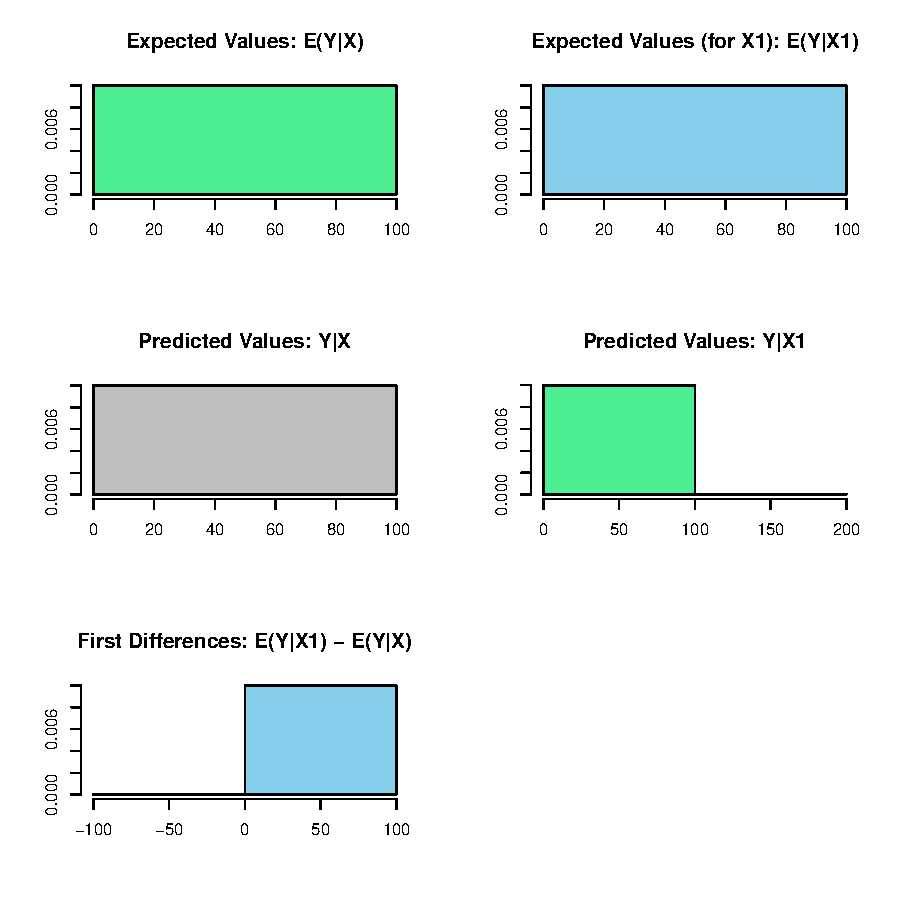
\includegraphics{vigpics/gamma-ExamplePlot}
\end{center}

\subsubsection{Model}

\begin{itemize}
\item The Gamma distribution with scale parameter $\alpha$ has a
\emph{stochastic component}:
\begin{eqnarray*}
Y &\sim& \textrm{Gamma}(y_i \mid \lambda_i, \alpha) \\
f(y)  &=& \frac{1}{\alpha^{\lambda_i} \, \Gamma \lambda_i} \, y_i^{\lambda_i
  - 1} \exp -\left\{ \frac{y_i}{\alpha} \right\}
\end{eqnarray*}
for $\alpha, \lambda_i, y_i > 0$.  \\

\item The \emph{systematic component} is given by
\begin{equation*}
  \lambda_i = \frac{1}{x_i \beta}
\end{equation*}
\end{itemize}

\subsubsection{Quantities of Interest}

\begin{itemize}
\item The expected values ({\tt qi\$ev}) are simulations of the mean
  of the stochastic component given draws of $\alpha$ and
  $\beta$ from their posteriors:  $$E(Y) = \alpha \lambda_i.$$  
\item The predicted values ({\tt qi\$pr}) are draws from the gamma
  distribution for each given set of parameters $(\alpha, \lambda_i)$.
\item If {\tt x1} is specified, {\tt sim()} also returns the
  differences in the expected values ({\tt qi\$fd}), $$E(Y \mid x_1) -
  E(Y \mid x)$$.

\item In conditional prediction models, the average expected treatment
  effect ({\tt att.ev}) for the treatment group is 
    \begin{equation*} \frac{1}{\sum_{i=1}^n t_i}\sum_{i:t_i=1}^n \left\{ Y_i(t_i=1) -
      E[Y_i(t_i=0)] \right\},
    \end{equation*} 
    where $t_i$ is a binary explanatory variable defining the treatment
    ($t_i=1$) and control ($t_i=0$) groups.  Variation in the
    simulations are due to uncertainty in simulating $E[Y_i(t_i=0)]$,
    the counterfactual expected value of $Y_i$ for observations in the
    treatment group, under the assumption that everything stays the
    same except that the treatment indicator is switched to $t_i=0$.

\item In conditional prediction models, the average predicted treatment
  effect ({\tt att.pr}) for the treatment group is 
    \begin{equation*} \frac{1}{\sum_{i=1}^n t_i}\sum_{i:t_i=1}^n \left\{ Y_i(t_i=1) -
      \widehat{Y_i(t_i=0)} \right\},
    \end{equation*} 
    where $t_i$ is a binary explanatory variable defining the treatment
    ($t_i=1$) and control ($t_i=0$) groups.  Variation in the
    simulations are due to uncertainty in simulating
    $\widehat{Y_i(t_i=0)}$, the counterfactual predicted value of
    $Y_i$ for observations in the treatment group, under the
    assumption that everything stays the same except that the
    treatment indicator is switched to $t_i=0$.  

\end{itemize}

\subsubsection{Output Values}

The output of each Zelig command contains useful information which you
may view.  For example, if you run \texttt{z.out <- zelig(y \~\,
  x, model = "gamma", data)}, then you may examine the available
information in \texttt{z.out} by using \texttt{names(z.out)},
see the {\tt coefficients} by using {\tt z.out\$coefficients}, and
a default summary of information through \texttt{summary(z.out)}.
Other elements available through the {\tt \$} operator are listed
below.

\begin{itemize}
\item From the {\tt zelig()} output object {\tt z.out}, you may
  extract:
   \begin{itemize}
   \item {\tt coefficients}: parameter estimates for the explanatory
     variables.
   \item {\tt residuals}: the working residuals in the final iteration
     of the IWLS fit.
   \item {\tt fitted.values}: the vector of fitted values.
   \item {\tt linear.predictors}: the vector of $x_{i}\beta$.
   \item {\tt aic}: Akaike's Information Criterion (minus twice the
     maximized log-likelihood plus twice the number of coefficients).
   \item {\tt df.residual}: the residual degrees of freedom.
   \item {\tt df.null}: the residual degrees of freedom for the null
     model.
   \item {\tt zelig.data}: the input data frame if {\tt save.data = TRUE}.  
   \end{itemize}

\item From {\tt summary(z.out)}, you may extract: 
   \begin{itemize}
   \item {\tt coefficients}: the parameter estimates with their
     associated standard errors, $p$-values, and $t$-statistics.
   \item{\tt cov.scaled}: a $k \times k$ matrix of scaled covariances.
   \item{\tt cov.unscaled}: a $k \times k$ matrix of unscaled
     covariances.  
   \end{itemize}

\item From the {\tt sim()} output object {\tt s.out}, you may extract
  quantities of interest arranged as matrices indexed by simulation
  $\times$ {\tt x}-observation (for more than one {\tt x}-observation).
  Available quantities are:

   \begin{itemize}
   \item {\tt qi\$ev}: the simulated expected values for the specified
     values of {\tt x}.
   \item {\tt qi\$pr}: the simulated predicted values drawn from a
     distribution defined by $(\alpha, \lambda_i)$.
   \item {\tt qi\$fd}: the simulated first difference in the expected
     values for the specified values in {\tt x} and {\tt x1}.
   \item {\tt qi\$att.ev}: the simulated average expected treatment
     effect for the treated from conditional prediction models.  
   \item {\tt qi\$att.pr}: the simulated average predicted treatment
     effect for the treated from conditional prediction models.  
   \end{itemize}
\end{itemize}


\subsection* {How to Cite} 


\CiteZelig

\subsection* {See also}
The gamma model is part of the stats package by \citet{VenRip02}.
Advanced users may wish to refer to \texttt{help(glm)} and
\texttt{help(family)}, as well as \cite{McCNel89}. Robust standard
errors are implemented via the sandwich package by \citet{Zeileis04}.
Sample data are from \cite{KinTomWit00}.

\bibliographystyle{asa}
\bibliography{gk,gkpubs}
 \end{document}


%%% Local Variables: 
%%% mode: latex
%%% TeX-master: t
%%% End: 









